\documentclass[11pt]{article}

\usepackage{amsmath}
\usepackage{mathtools}
\usepackage{times}
\usepackage{enumerate}
\usepackage[makeroom]{cancel}
\usepackage{cite}
\usepackage[usenames, dvipsnames]{color}
\usepackage{textpos}
\usepackage[pdftex]{graphicx}
\usepackage{subfigure}	
\usepackage{amssymb}  % assumes amsmath package installed 
\usepackage{color} % Farbiger text
\usepackage{pifont}
\usepackage[abs]{overpic}
\usepackage{xcolor,varwidth}
\DeclareGraphicsExtensions{.pdf,.jpg,.png,.eps}
\usepackage{url}
\usepackage[normalem]{ulem}
\usepackage{cancel}
\usepackage{xcolor}
\usepackage{soul}



\newcommand{\mathcolorbox}[2]{\colorbox{#1}{$\displaystyle #2$}}
\newcommand{\zutun}[1]{\textcolor{red}{\textbf{#1}}}
\newcommand{\vect}[1]{\boldsymbol{#1}}
\newcommand{\cmark}{\textcolor{green}{\ding{51}}}%
\newcommand{\xmark}{\textcolor{red}{\ding{55}}}%
\newcommand{\grad}{$^\circ$}%

\newtheorem{mydef}{Theorem}



%
\makeatletter
\date{}
%
%\@ifundefined{showcaptionsetup}{}{%
% \PassOptionsToPackage{caption=false}{subfig}}
%\usepackage{subfig}
%\makeatother
%

%
\begin{document}
%
\title{Should we really use $\bar{\vect{q}}$? 
\footnotesize }
\maketitle
%
\section{Spring-mass}
\subsection{The system}
\begin{center}
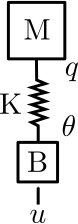
\includegraphics[scale=0.6]{drawing.pdf} 
\end{center}
Dynamics equation: 
\begin{align}
u - K(\theta-q) &= B \ddot{\theta} \\
K(\theta - q) &= M \ddot{q} + g(q)
\end{align}
Defining desired motor side position according to link side position: 
\begin{equation}
K(\theta_d-q_d) = M\ddot{q}_d 
\end{equation}
Control input:
\begin{align}
u &= - K_q \tilde{q} - D_q \dot{\tilde{q}} + M \ddot{q}_d + B\ddot{\theta}_d + \hat{g}(q) \\
\tilde{q} &= q - q_d \nonumber
\end{align}

\subsection{Problem formulation}
Closed loop dynamics: 
\begin{align}
 M \ddot{q}_d + B\ddot{\theta}_d - B \ddot{\theta} - K_q \tilde{q} - D_q \dot{\tilde{q}} + \hat{g}(q)  = M \ddot{q} + g(q)
\end{align}
Power balance equation with flow $\dot{\theta}$: 
\begin{align}
\underbrace{\dot{\theta}\underbrace{M \ddot{q}_d}_{K(\theta_d-q_d)}}_{\dot{q}\underbrace{K(\theta_d-q_d)}_{M\ddot{q}_d} + (\dot{\theta}-\dot{q})K(\theta_d-q_d)} + \dot{\theta}B\ddot{\theta}_d - \dot{\theta}B \ddot{\theta} - \dot{\theta}(K_q \tilde{q} + D_q \dot{\tilde{q}}) + \dot{\theta}\hat{g}(q) = \underbrace{\dot{\theta}\underbrace{(M \ddot{q} + g(q))}_{K(\theta-q)}}_{\dot{q}\underbrace{K(\theta-q)}_{M\ddot{q}+g(q)}+(\dot{\theta}-\dot{q})K(\theta-q)} \label{eq:closedLoopTheta}
\end{align}
Power balance equation with flow $\dot{\theta}_d$: 
\begin{align}
\underbrace{\dot{\theta}_d\underbrace{M \ddot{q}_d}_{K(\theta_d-q_d)}}_{\dot{q}_d\underbrace{K(\theta_d-q_d)}_{M\ddot{q}_d} + (\dot{\theta}_d-\dot{q}_d)K(\theta_d-q_d)} + \dot{\theta}_dB\ddot{\theta}_d - \dot{\theta}_dB \ddot{\theta} - \dot{\theta}_d(K_q \tilde{q} + D_q \dot{\tilde{q}}) + \dot{\theta}_d\hat{g}(q) = \underbrace{\dot{\theta}_d\underbrace{(M \ddot{q} + g(q))}_{K(\theta-q)}}_{\dot{q}_d\underbrace{K(\theta-q)}_{M\ddot{q}+g(q)}+(\dot{\theta}_d-\dot{q}_d)K(\theta-q)} \label{eq:closedLoopThetaD}
\end{align}
Subtracting (\ref{eq:closedLoopTheta}) from (\ref{eq:closedLoopThetaD}):
\begin{align}
\dot{\tilde{q}}M\dot{\tilde{q}} + \dot{\tilde{\theta}}B\dot{\tilde{\theta}} + \underbrace{\dot{\tilde{\theta}}K_q\tilde{q}}_{ \stackrel{?}{=} \dot{S}} \underbrace{- \dot{\tilde{\theta}}\hat{g}(q) + \dot{\tilde{q}}g(q)}_{ \stackrel{?}{=} \dot{S}/0} = -\underbrace{\dot{\tilde{\theta}}D_q\dot{\tilde{q}}}_{ \stackrel{?}{=} P_D} \label{eq:closedLoop}
\end{align} 
\subsection{Only regulation and Albu-schaeffer idea}
Closed loop dynamics (\ref{eq:closedLoop}) will boil down to: 
\begin{align}
\dot{q}M\dot{q} + \dot{\theta}B\dot{\theta} + \dot{\theta}K_q\tilde{q} - \dot{\theta}\hat{g}(q) + \dot{q}g(q) = -\dot{\theta}D_q\dot{q}
\end{align}

\bibliography{mybib}{}
%\bibliographystyle{plain}
\end{document}
